\documentclass[10pt,aspectratio=169]{beamer}
\usetheme{Madrid}
\setbeamertemplate{navigation symbols}{}

\usepackage[T1]{fontenc}
\usepackage[utf8]{inputenc}
\usepackage{lmodern}
\usepackage{amsmath}
\usepackage{booktabs}
\usepackage{graphicx}
\usepackage{xcolor}
\usepackage{tikz}
\usetikzlibrary{positioning,arrows.meta}

\definecolor{Ink}{HTML}{16324F}
\definecolor{Accent}{HTML}{E76F51}
\definecolor{Soft}{HTML}{F3F0E8}
\definecolor{Deep}{HTML}{102A43}
\definecolor{Good}{HTML}{2A9D8F}

\setbeamercolor{title}{fg=white,bg=Ink}
\setbeamercolor{frametitle}{fg=white,bg=Ink}
\setbeamercolor{structure}{fg=Ink}
\setbeamercolor{block title}{fg=white,bg=Ink}
\setbeamercolor{block body}{fg=black,bg=Soft}
\setbeamercolor{itemize item}{fg=Accent}
\setbeamercolor{enumerate item}{fg=Accent}

\newcommand{\callout}[1]{%
  \begin{beamercolorbox}[rounded=true,shadow=true,sep=0.9em,wd=\linewidth]{block body}
  \centering \Large \textbf{#1}
  \end{beamercolorbox}
}

\newcommand{\smallcallout}[1]{%
  \begin{beamercolorbox}[rounded=true,shadow=false,sep=0.7em,wd=\linewidth]{block body}
  \centering \normalsize \textbf{#1}
  \end{beamercolorbox}
}

\newcommand{\statcard}[2]{%
  \begin{beamercolorbox}[rounded=true,shadow=true,sep=0.7em,wd=\linewidth]{block body}
  \centering
  {\color{Accent}\fontsize{20}{22}\selectfont \textbf{#1}}\\[0.3em]
  {\small #2}
  \end{beamercolorbox}
}

\title{Do LLM Rankings Change if You Ask Differently?}
\subtitle{A 10-minute walk through ranking reversals under prompt perturbations}
\author{ST5230 Group 14\\ZHANG QIANCHI \and PENG YANGYUNZHI \and JIANG YIFAN \and MENG XIANGCHEN}
\date{}

\begin{document}

\begin{frame}[plain]
  \begin{tikzpicture}[remember picture,overlay]
    \fill[Ink] (current page.south west) rectangle (current page.north east);
  \end{tikzpicture}
  \vspace{1.2cm}
  {\color{white}\Huge \textbf{Do LLM Rankings Change}}\\[0.15cm]
  {\color{white}\Huge \textbf{if You Ask Differently?}}\\[0.5cm]
  {\color{white}\large Ranking reversals under non-semantic prompt perturbations}\\[0.1cm]
  {\color{white}\large and subset resampling}\\[1.1cm]
  {\color{white}\normalsize ST5230 Group 14}
\end{frame}

\begin{frame}{The Question We Usually Ignore}
  \begin{columns}[T]
    \begin{column}{0.48\textwidth}
      \begin{beamercolorbox}[rounded=true,shadow=true,sep=0.9em,wd=\linewidth]{block body}
        {\Large \textbf{What a leaderboard says}}\\[0.6em]
        \begin{itemize}
          \item Model A: 89.2\%
          \item Model B: 87.3\%
          \item Therefore, A $>$ B
        \end{itemize}
      \end{beamercolorbox}
    \end{column}
    \begin{column}{0.48\textwidth}
      \begin{beamercolorbox}[rounded=true,shadow=true,sep=0.9em,wd=\linewidth]{block body}
        {\Large \textbf{What we ask instead}}\\[0.6em]
        \begin{itemize}
          \item What if we change the prompt wording?
          \item What if we sample a different subset?
          \item Does A still beat B?
        \end{itemize}
      \end{beamercolorbox}
    \end{column}
  \end{columns}

  \vspace{0.8em}
  \callout{Our object of study is not only score, but ranking stability.}
\end{frame}

\begin{frame}{Why This Matters}
  \begin{columns}[T]
    \begin{column}{0.33\textwidth}
      \statcard{Static leaderboards}{convenient, but treated as if they were stable facts}
    \end{column}
    \begin{column}{0.33\textwidth}
      \statcard{Prompt wording}{can change how a model interprets the same task}
    \end{column}
    \begin{column}{0.33\textwidth}
      \statcard{Subset choice}{can change the apparent winner when gaps are small}
    \end{column}
  \end{columns}

  \vspace{0.9em}
  \smallcallout{If rank changes under reasonable evaluation choices, a single leaderboard is not the whole story.}
\end{frame}

\begin{frame}{Related Work, and Our Gap}
  \begin{columns}[T]
    \begin{column}{0.31\textwidth}
      \statcard{Benchmarks}{MMLU, ARC, and HellaSwag define the evaluation settings.}
    \end{column}
    \begin{column}{0.31\textwidth}
      \statcard{Prompt robustness}{prior work shows that task-preserving prompt changes can matter.}
    \end{column}
    \begin{column}{0.31\textwidth}
      \statcard{Evaluation reliability}{recent discussions argue protocol matters, not just the model.}
    \end{column}
  \end{columns}

  \vspace{0.9em}
  \callout{Missing piece: can small evaluation changes actually flip the model order?}
\end{frame}

\begin{frame}{Our Idea}
  \begin{columns}[T]
    \begin{column}{0.56\textwidth}
      \begin{itemize}
        \item Keep the task fixed.
        \item Perturb the prompt in a non-semantic, task-preserving way.
        \item Bootstrap the evaluation subset.
        \item Observe whether the induced ranking changes.
      \end{itemize}

      \vspace{0.6em}
      \[
      \text{RRR} = \Pr(\text{ranking differs from the minimal prompt baseline})
      \]

      \vspace{0.4em}
      \begin{itemize}
        \item Low RRR: the leaderboard is robust
        \item High RRR: the leaderboard is fragile
      \end{itemize}
    \end{column}
    \begin{column}{0.4\textwidth}
      \begin{beamercolorbox}[rounded=true,shadow=true,sep=0.9em,wd=\linewidth]{block body}
        {\large \textbf{Interpretation}}\\[0.5em]
        We treat rank as a random outcome induced by evaluation choices, not as a fixed property.
      \end{beamercolorbox}
    \end{column}
  \end{columns}
\end{frame}

\begin{frame}{From Data to Ranking Reversal}
  \centering
  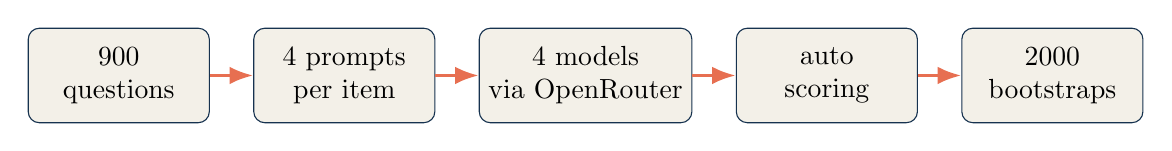
\begin{tikzpicture}[
      node distance=0.55cm,
      box/.style={draw=Ink, fill=Soft, rounded corners, minimum height=1.2cm, minimum width=2.3cm, align=center},
      arr/.style={-{Latex[length=3mm]}, very thick, draw=Accent}
    ]
    \node[box] (q) {900\\questions};
    \node[box, right=of q] (p) {4 prompts\\per item};
    \node[box, right=of p] (m) {4 models\\via OpenRouter};
    \node[box, right=of m] (s) {auto\\scoring};
    \node[box, right=of s] (b) {2000\\bootstraps};

    \draw[arr] (q) -- (p);
    \draw[arr] (p) -- (m);
    \draw[arr] (m) -- (s);
    \draw[arr] (s) -- (b);
  \end{tikzpicture}

  \vspace{1em}
  \begin{columns}[T]
    \begin{column}{0.24\textwidth}
      \statcard{3600}{prompt requests}
    \end{column}
    \begin{column}{0.24\textwidth}
      \statcard{14400}{model responses}
    \end{column}
    \begin{column}{0.24\textwidth}
      \statcard{3}{parse failures only}
    \end{column}
    \begin{column}{0.24\textwidth}
      \statcard{0.02\%}{failure rate}
    \end{column}
  \end{columns}
\end{frame}

\begin{frame}{First Big Result: Stability Depends on the Benchmark}
  \begin{columns}[T]
    \begin{column}{0.62\textwidth}
      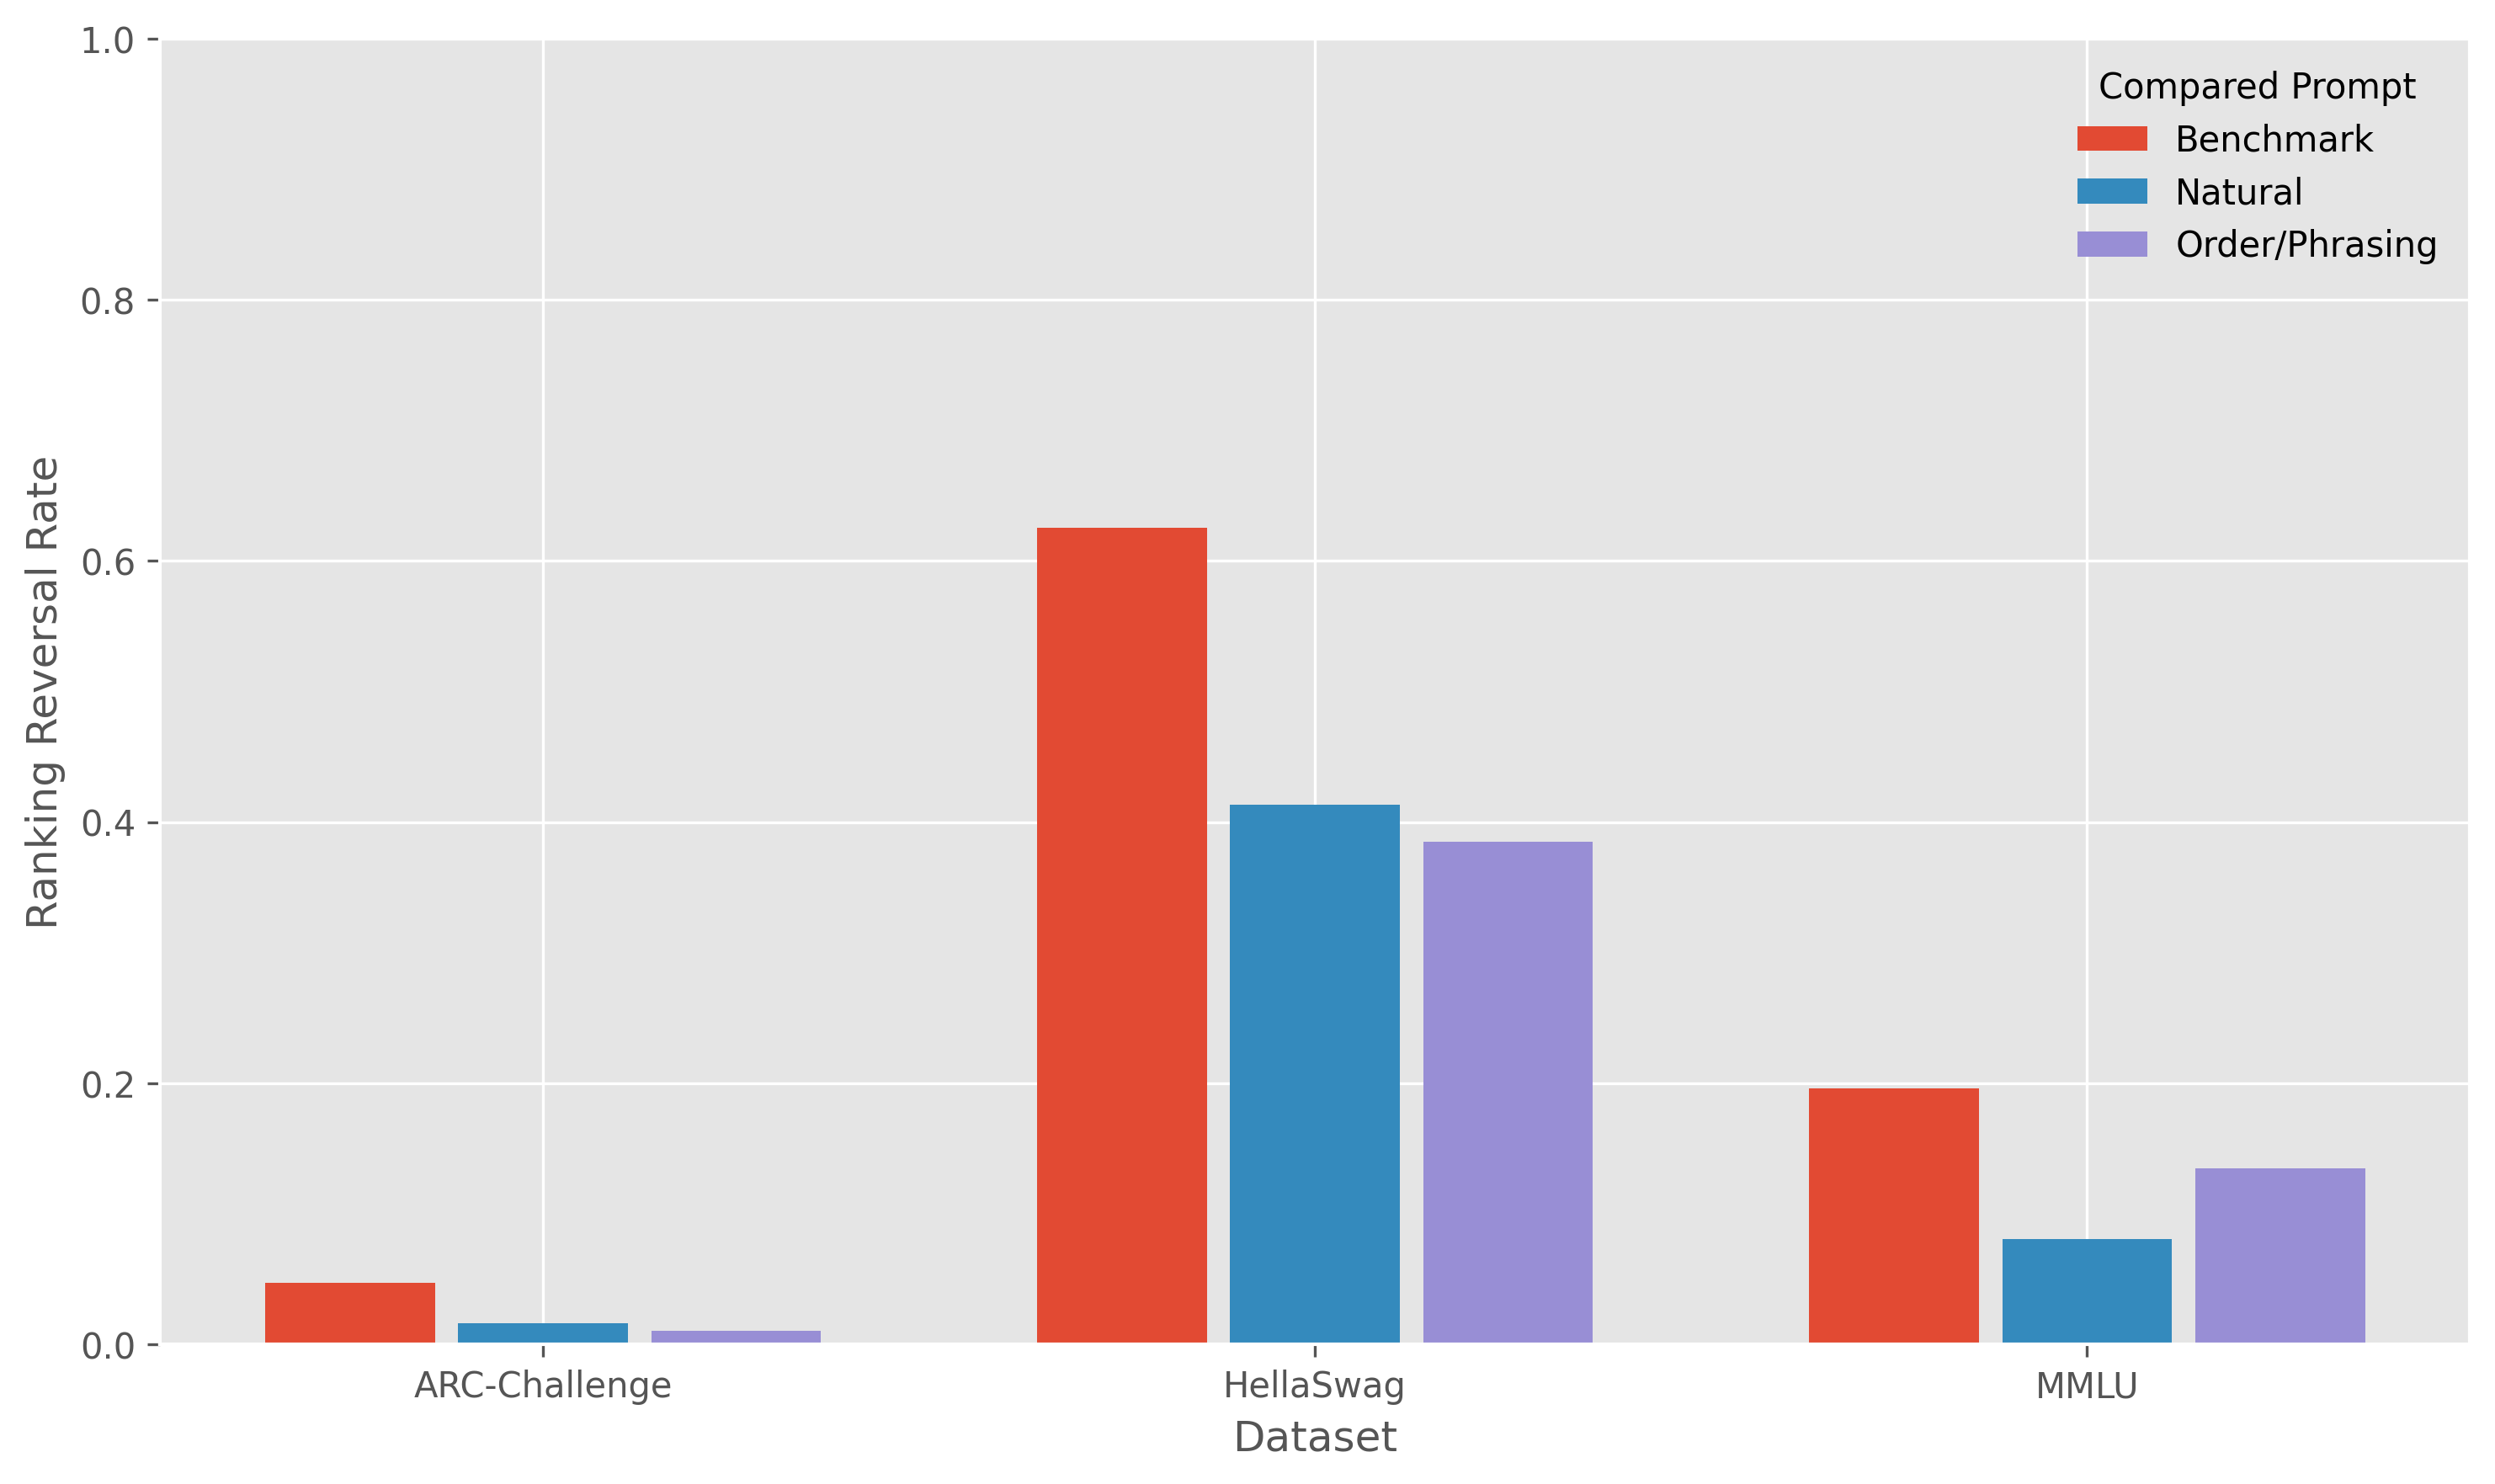
\includegraphics[width=\linewidth]{figures/ranking_reversal_rate.png}
    \end{column}
    \begin{column}{0.35\textwidth}
      \statcard{ARC}{Very stable}
      \vspace{0.35em}
      \statcard{MMLU}{Moderately stable}
      \vspace{0.35em}
      \statcard{HellaSwag}{Highly fragile}
    \end{column}
  \end{columns}

  \vspace{0.5em}
  \smallcallout{The same evaluation idea produces radically different ranking stability across benchmarks.}
\end{frame}

\begin{frame}{Case Study: HellaSwag Breaks the Static Leaderboard Story}
  \begin{columns}[T]
    \begin{column}{0.33\textwidth}
      \statcard{62.55\%}{highest RRR under the benchmark-style prompt}
    \end{column}
    \begin{column}{0.33\textwidth}
      \statcard{1.92\%}{GPT lead over Gemini in prompt-averaged accuracy}
    \end{column}
    \begin{column}{0.33\textwidth}
      \statcard{$p=0.169$}{the GPT--Gemini gap is not statistically significant}
    \end{column}
  \end{columns}

  \vspace{0.9em}
  \begin{beamercolorbox}[rounded=true,shadow=true,sep=0.9em,wd=\linewidth]{block body}
    \centering
    \Large \textbf{Conclusion for HellaSwag:}\\[0.3em]
    GPT looks first by point estimate, but the top rank is not secure once prompt and subset variation are taken seriously.
  \end{beamercolorbox}
\end{frame}

\begin{frame}{Contrast: ARC and MMLU Tell a More Nuanced Story}
  \begin{columns}[T]
    \begin{column}{0.48\textwidth}
      \begin{beamercolorbox}[rounded=true,shadow=true,sep=0.9em,wd=\linewidth]{block body}
        {\Large \textbf{ARC-Challenge}}\\[0.5em]
        \begin{itemize}
          \item Gemini is clearly first.
          \item All pairwise gaps are significant.
          \item RRR stays near zero.
        \end{itemize}
        \vspace{0.4em}
        \textbf{Interpretation:} leaderboard is genuinely robust.
      \end{beamercolorbox}
    \end{column}
    \begin{column}{0.48\textwidth}
      \begin{beamercolorbox}[rounded=true,shadow=true,sep=0.9em,wd=\linewidth]{block body}
        {\Large \textbf{MMLU}}\\[0.5em]
        \begin{itemize}
          \item Gemini is also clearly first.
          \item But GPT vs Qwen is not significant.
          \item Instability sits in the middle ranks.
        \end{itemize}
        \vspace{0.4em}
        \textbf{Interpretation:} stable winner, less stable ordering below.
      \end{beamercolorbox}
    \end{column}
  \end{columns}
\end{frame}

\begin{frame}{One More Layer: Even MMLU Is Not Uniform}
  \begin{columns}[T]
    \begin{column}{0.62\textwidth}
      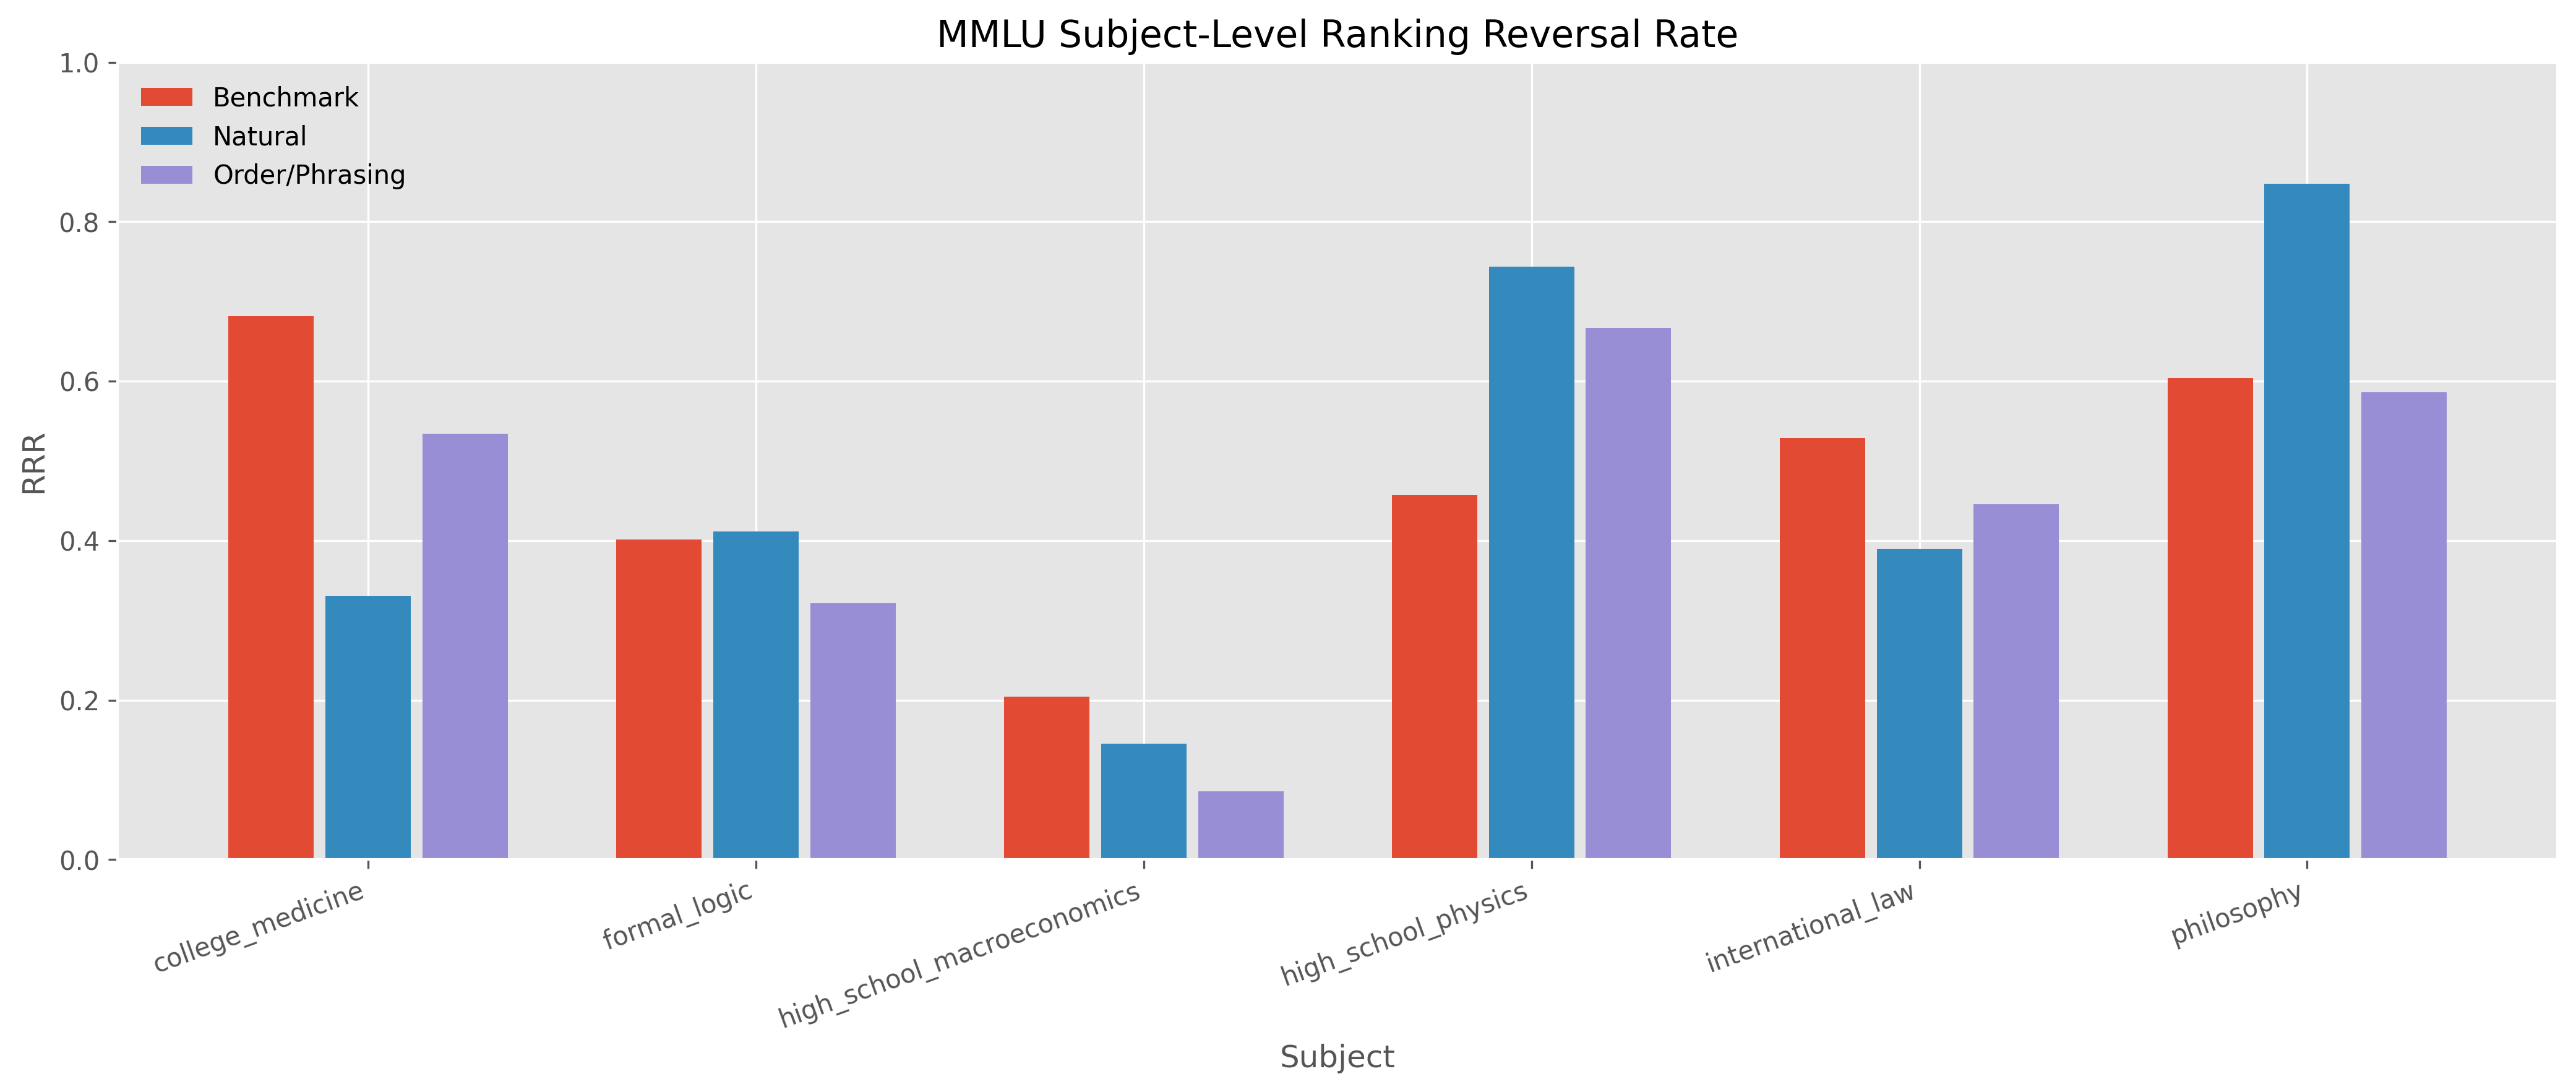
\includegraphics[width=\linewidth]{figures/mmlu_subject_rrr.png}
    \end{column}
    \begin{column}{0.35\textwidth}
      \begin{itemize}
        \item Full MMLU keeps the same overall winner.
        \item Subject-level RRR varies a lot.
        \item Mean non-minimal RRR ranges from about 14.5\% to 67.9\%.
      \end{itemize}

      \vspace{0.6em}
      \smallcallout{Ranking robustness is not only benchmark-dependent, but also subdomain-dependent.}
    \end{column}
  \end{columns}
\end{frame}

\begin{frame}{What Does This Project Show?}
  \begin{columns}[T]
    \begin{column}{0.32\textwidth}
      \statcard{What we did}{measured ranking stability instead of reporting only average accuracy}
    \end{column}
    \begin{column}{0.32\textwidth}
      \statcard{What we found}{rankings can be robust, partially stable, or fragile depending on the task}
    \end{column}
    \begin{column}{0.32\textwidth}
      \statcard{What it means}{a trustworthy benchmark report should include uncertainty and rank robustness}
    \end{column}
  \end{columns}

  \vspace{1em}
  \callout{The real question is not only ``Who is best?'' but ``Does that ordering survive reasonable evaluation variation?''}
\end{frame}

\end{document}
